% Configuração do tipo de documento
\documentclass{article}

% Configuração do idioma
\usepackage[utf8]{inputenc}
\usepackage{lipsum}
\usepackage{graphics}
\usepackage{tcolorbox}
\usepackage{helvet}
\usepackage{setspace}

% Configuração da fonte e espaçamento - Abnt
\renewcommand{\familydefault}{\sfdefault}
\onehalfspacing

% Configuração do título
\title{\bfseries\fontsize{16}{16}\selectfont Título do Artigo}
\author{}
\date{}

% Configuração do cabeçalho e rodapé
\usepackage{fancyhdr}
\pagestyle{fancy}
\fancyhf{}
\rhead{Nome do Autor}
\lhead{Título do Artigo}
\rfoot{Página \thepage}

% Início do documento
\begin{document}

% Adição de imagem
\begin{figure}[h]
    \centering
    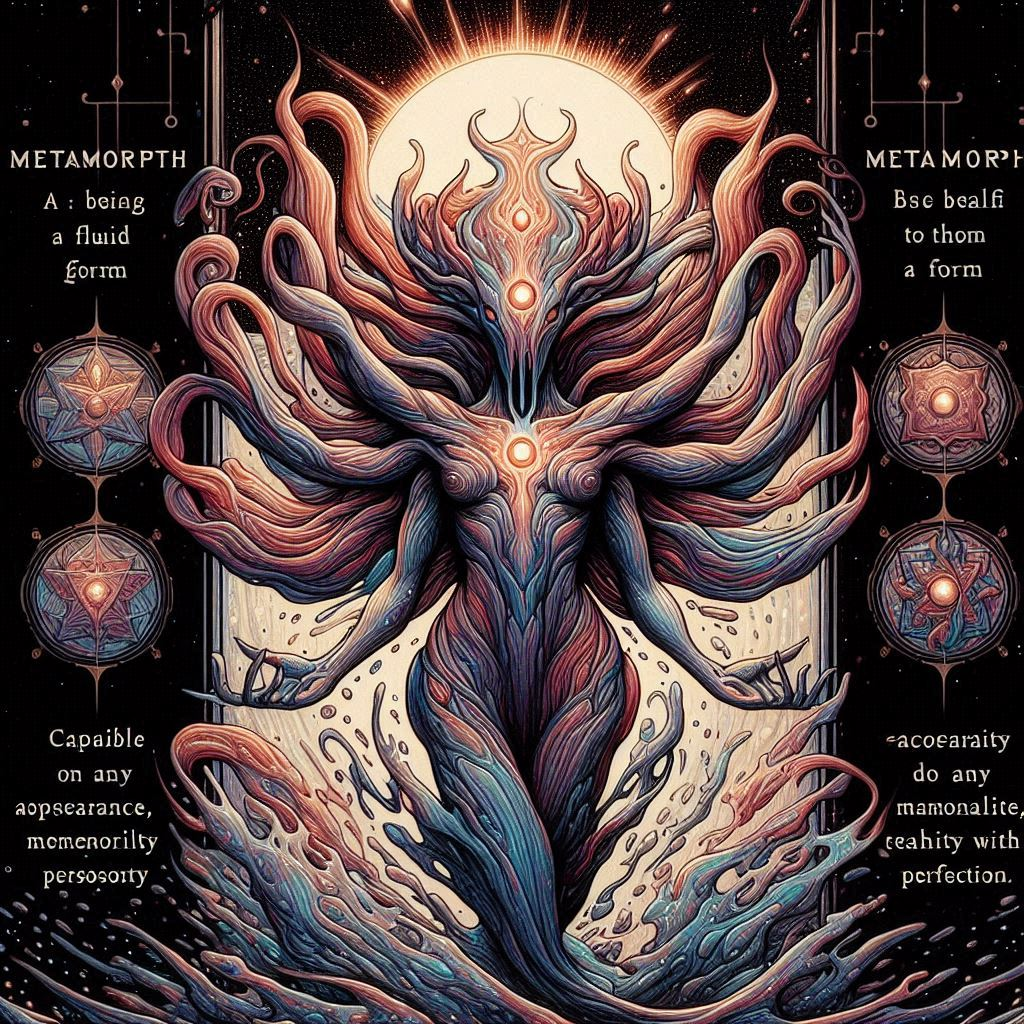
\includegraphics[width=0.5\textwidth]{Metamorph_All.jpeg}
    \maketitle
\end{figure}
\newpage

% Inclusão do sumário
\renewcommand{\contentsname}{Sumário}
\tableofcontents
\newpage

% Inclusão de seção
\section{Introdução}
\lipsum[1]

% Inclusão de tabela
\begin{table}[h]
    \centering
    \begin{tabular}{|c|c|c|}
        \hline
        Coluna 1 & Coluna 2 & Coluna 3 \\
        \hline
        1 & 2 & 3 \\
        \hline
        4 & 5 & 6 \\
        \hline
        7 & 8 & 9 \\
        \hline
    \end{tabular}
    \caption{Exemplo de tabela}
\end{table}

% Inclusão de seção
\section{Desenvolvimento}
\lipsum[2]

% Inclusão de tópico
\subsection{Sub-tópico 1}
\lipsum[1]

% Inclusão de sub-tópico
\subsubsection{Subsub-tópico 1}
\lipsum[1]

% Inclusão de sub-tópico
\subsubsection{Subsub-tópico 2}
\lipsum[1]

% Inclusão de tópico
\subsection{Sub-tópico 2}
\lipsum[2]

% Inclusão de tópico
\subsection{Sub-tópico 3}
\lipsum[3]

% Inclusão de lista não enumerada
\begin{itemize}
    \item Item 1
    \begin{itemize}
        \item Subitem 1
        \item Subitem 2
        \begin{itemize}
            \item Subsubitem 1
            \item Subsubitem 2
        \end{itemize}
    \end{itemize}
    \item Item 2
    \item Item 3
\end{itemize}

% Inclusão de seção
\section{Conclusão}
\lipsum[3]

% Inclusão de lista enumerada
\begin{enumerate}
    \item Item 1
    \begin{enumerate}
        \item Subitem 1
        \item Subitem 2
        \begin{enumerate}
            \item Subsubitem 1
            \item Subsubitem 2
        \end{enumerate}
    \end{enumerate}
    \item Item 2
    \item Item 3
\end{enumerate}

% Fim do documento
\end{document}